\documentclass[conference]{IEEEtran}
\IEEEoverridecommandlockouts
\usepackage{cite}
\usepackage{amsmath,amssymb,amsfonts}
\usepackage{algorithmic}
\usepackage{graphicx}
\usepackage[space]{grffile}
\usepackage{textcomp}
\usepackage{xcolor}
\usepackage{float}
\usepackage{listings}

\lstset{
    basicstyle=\ttfamily\scriptsize,
    breaklines=true,
    frame=single,
    backgroundcolor=\color{gray!10},
    keywordstyle=\color{blue},
    commentstyle=\color{gray},
    stringstyle=\color{red},
    numbers=none,
    tabsize=2,
    showstringspaces=false
}

\graphicspath{{image_tex/}}

\def\BibTeX{{\rm B\kern-.05em{\sc i\kern-.025em b}\kern-.08em
    T\kern-.1667em\lower.7ex\hbox{E}\kern-.125emX}}

\begin{document}

\title{SI-UMKM Jabar: Rancang Bangun Sistem Informasi dan Layanan Terpadu UMKM Jawa Barat}

\author{
\IEEEauthorblockN{1\textsuperscript{st} Vania Rahmawati}
\IEEEauthorblockA{\textit{PSDKU Lamongan D3 Teknik Informatika} \\
\textit{Politeknik Elektronika Negeri Surabaya} \\
Lamongan, Indonesia}
\and
\IEEEauthorblockN{2\textsuperscript{nd} Reva Fadillah Susetya}
\IEEEauthorblockA{\textit{PSDKU Lamongan D3 Teknik Informatika} \\
\textit{Politeknik Elektronika Negeri Surabaya} \\
Lamongan, Indonesia}
}

\maketitle

\begin{abstract}
Sektor Usaha Mikro, Kecil, dan Menengah (UMKM) memegang peranan krusial dalam pertumbuhan ekonomi Jawa Barat. Namun, publikasi data UMKM saat ini masih terfragmentasi dan disajikan dalam format tabular statis, sementara alur pelayanan pengajuan program bantuan, perizinan, dan pelatihan masih berjalan secara terpisah tanpa mekanisme pelacakan yang terpadu. Penelitian ini bertujuan merancang dan mengimplementasikan SI-UMKM Jabar, sebuah platform e-governance terpadu berbasis web yang memadukan visualisasi geografis interaktif dan layanan mandiri pelaku usaha. Sistem dibangun dengan arsitektur RESTful API menggunakan framework FastAPI dan basis data MySQL, yang mendukung digitalisasi verifikasi berkas secara langsung oleh administrator. Evaluasi performa sistem melalui uji beban menunjukkan backend mampu menangani hingga 50 pengguna simultan dengan tingkat latensi rendah dan stabilitas respon yang tinggi. Platform ini diharapkan dapat mempercepat alur birokrasi layanan serta mempermudah pemetaan potensi sebaran UMKM secara transparan.
\end{abstract}

\begin{IEEEkeywords}
SI-UMKM Jabar, E-Governance, FastAPI, Pemetaan UMKM, REST API, ReactJS
\end{IEEEkeywords}

\section{Pendahuluan}

\subsection{Latar Belakang}
Sektor Usaha Mikro, Kecil, dan Menengah (UMKM) merupakan penopang utama stabilitas ekonomi daerah Jawa Barat dengan populasi lebih dari 7,05 juta unit usaha [1], [2]. Perkembangan transparansi data pemerintah daerah melalui portal data terbuka mendorong optimalisasi tata kelola dan pemanfaatan informasi publik secara lebih luas [1], [3]. Namun, penyediaan data terbuka tersebut belum sepenuhnya diimbangi oleh saluran partisipasi yang interaktif serta keterpaduan tindak lanjut layanan administrasi [3], [4]. Publikasi data yang masih disajikan secara tabular statis menyulitkan para pelaku usaha, mitra bisnis, maupun penyalur barang dalam membaca potensi sebaran niaga secara kontekstual [1], [2].

Kondisi tersebut diperberat oleh saluran pengurusan program UMKM yang masih berjalan terpisah-pisah, mulai dari permohonan bantuan sarana modal, registrasi kurasi pelatihan, hingga perizinan legalitas [2], [4]. Ketiadaan pintu layanan terpusat membuat proses pengajuan minim fasilitas pelacakan status (\textit{tracking}) serta rentan terhadap kesalahan input data persyaratan administratif [3], [4]. Untuk menjawab persoalan ini, dibutuhkan keterpaduan sistem yang menyatukan transparansi data spasial dengan standarisasi alur pengajuan layanan publik dalam satu platform terpusat.

Berdasarkan permasalahan tersebut, penelitian ini mengusulkan SI-UMKM Jabar sebagai platform terintegrasi berbasis web yang memadukan visualisasi peta sebaran kategori usaha berkode warna dan digitalisasi layanan mandiri. Sistem menghubungkan pemohon secara langsung dengan panel verifikasi administrator melalui arsitektur backend FastAPI berkecepatan tinggi, integrasi formulir terstruktur, serta pelacakan status pengajuan secara \textit{real-time}. Pengujian keandalan backend dilakukan menggunakan uji beban Postman dengan 50 pengguna simultan, serta disiapkan instrumen evaluasi kepuasan pengguna mengadopsi model Technology Acceptance Model (TAM).

\section{Ease of Use}

\section{Prepare Your Paper Before Styling}

\section*{Acknowledgment}

\begin{thebibliography}{00}
\bibitem{jurnal_jik} A. S. R. Kurniawan, ``Rancang Bangun Sistem Informasi Pengelolaan dan Pemetaan Data UMKM Berbasis Web,'' \textit{Jurnal Inovasi Komputer (JIK)}, vol. 7, no. 2, hlm. 88--96, 2023.
\bibitem{jurnal_jei} M. F. Amin, ``Strategi Digitalisasi Pelaku Usaha Mikro Kecil Menengah dalam Meningkatkan Daya Saing Perekonomian Daerah,'' \textit{Jurnal Ekonomi dan Kewirausahaan (JEI)}, vol. 14, no. 1, hlm. 45--56, 2024.
\bibitem{jurnal_jitet} R. Firmansyah dan E. Utami, ``Rancang Bangun Sistem Informasi Pelayanan Publik Berbasis Web Menggunakan Pendekatan Framework Modern,'' \textit{Jurnal Informatika dan Sistem Komputer (JITET)}, vol. 11, no. 2, hlm. 201--210, 2023.
\bibitem{jurnal_cc} H. Subowo, ``Implementasi E-Government dalam Peningkatan Kualitas Layanan Administrasi Publik pada Instansi Pemerintahan Daerah,'' \textit{CosmoGov: Jurnal Ilmu Pemerintahan}, vol. 9, no. 1, hlm. 35--48, 2023.
\end{thebibliography}

% ================= HALAMAN KHUSUS GAMBAR (1 HALAMAN 1 GAMBAR) =================
\clearpage
\onecolumn

\section{Architecture System}
\begin{figure}[H]
\centering
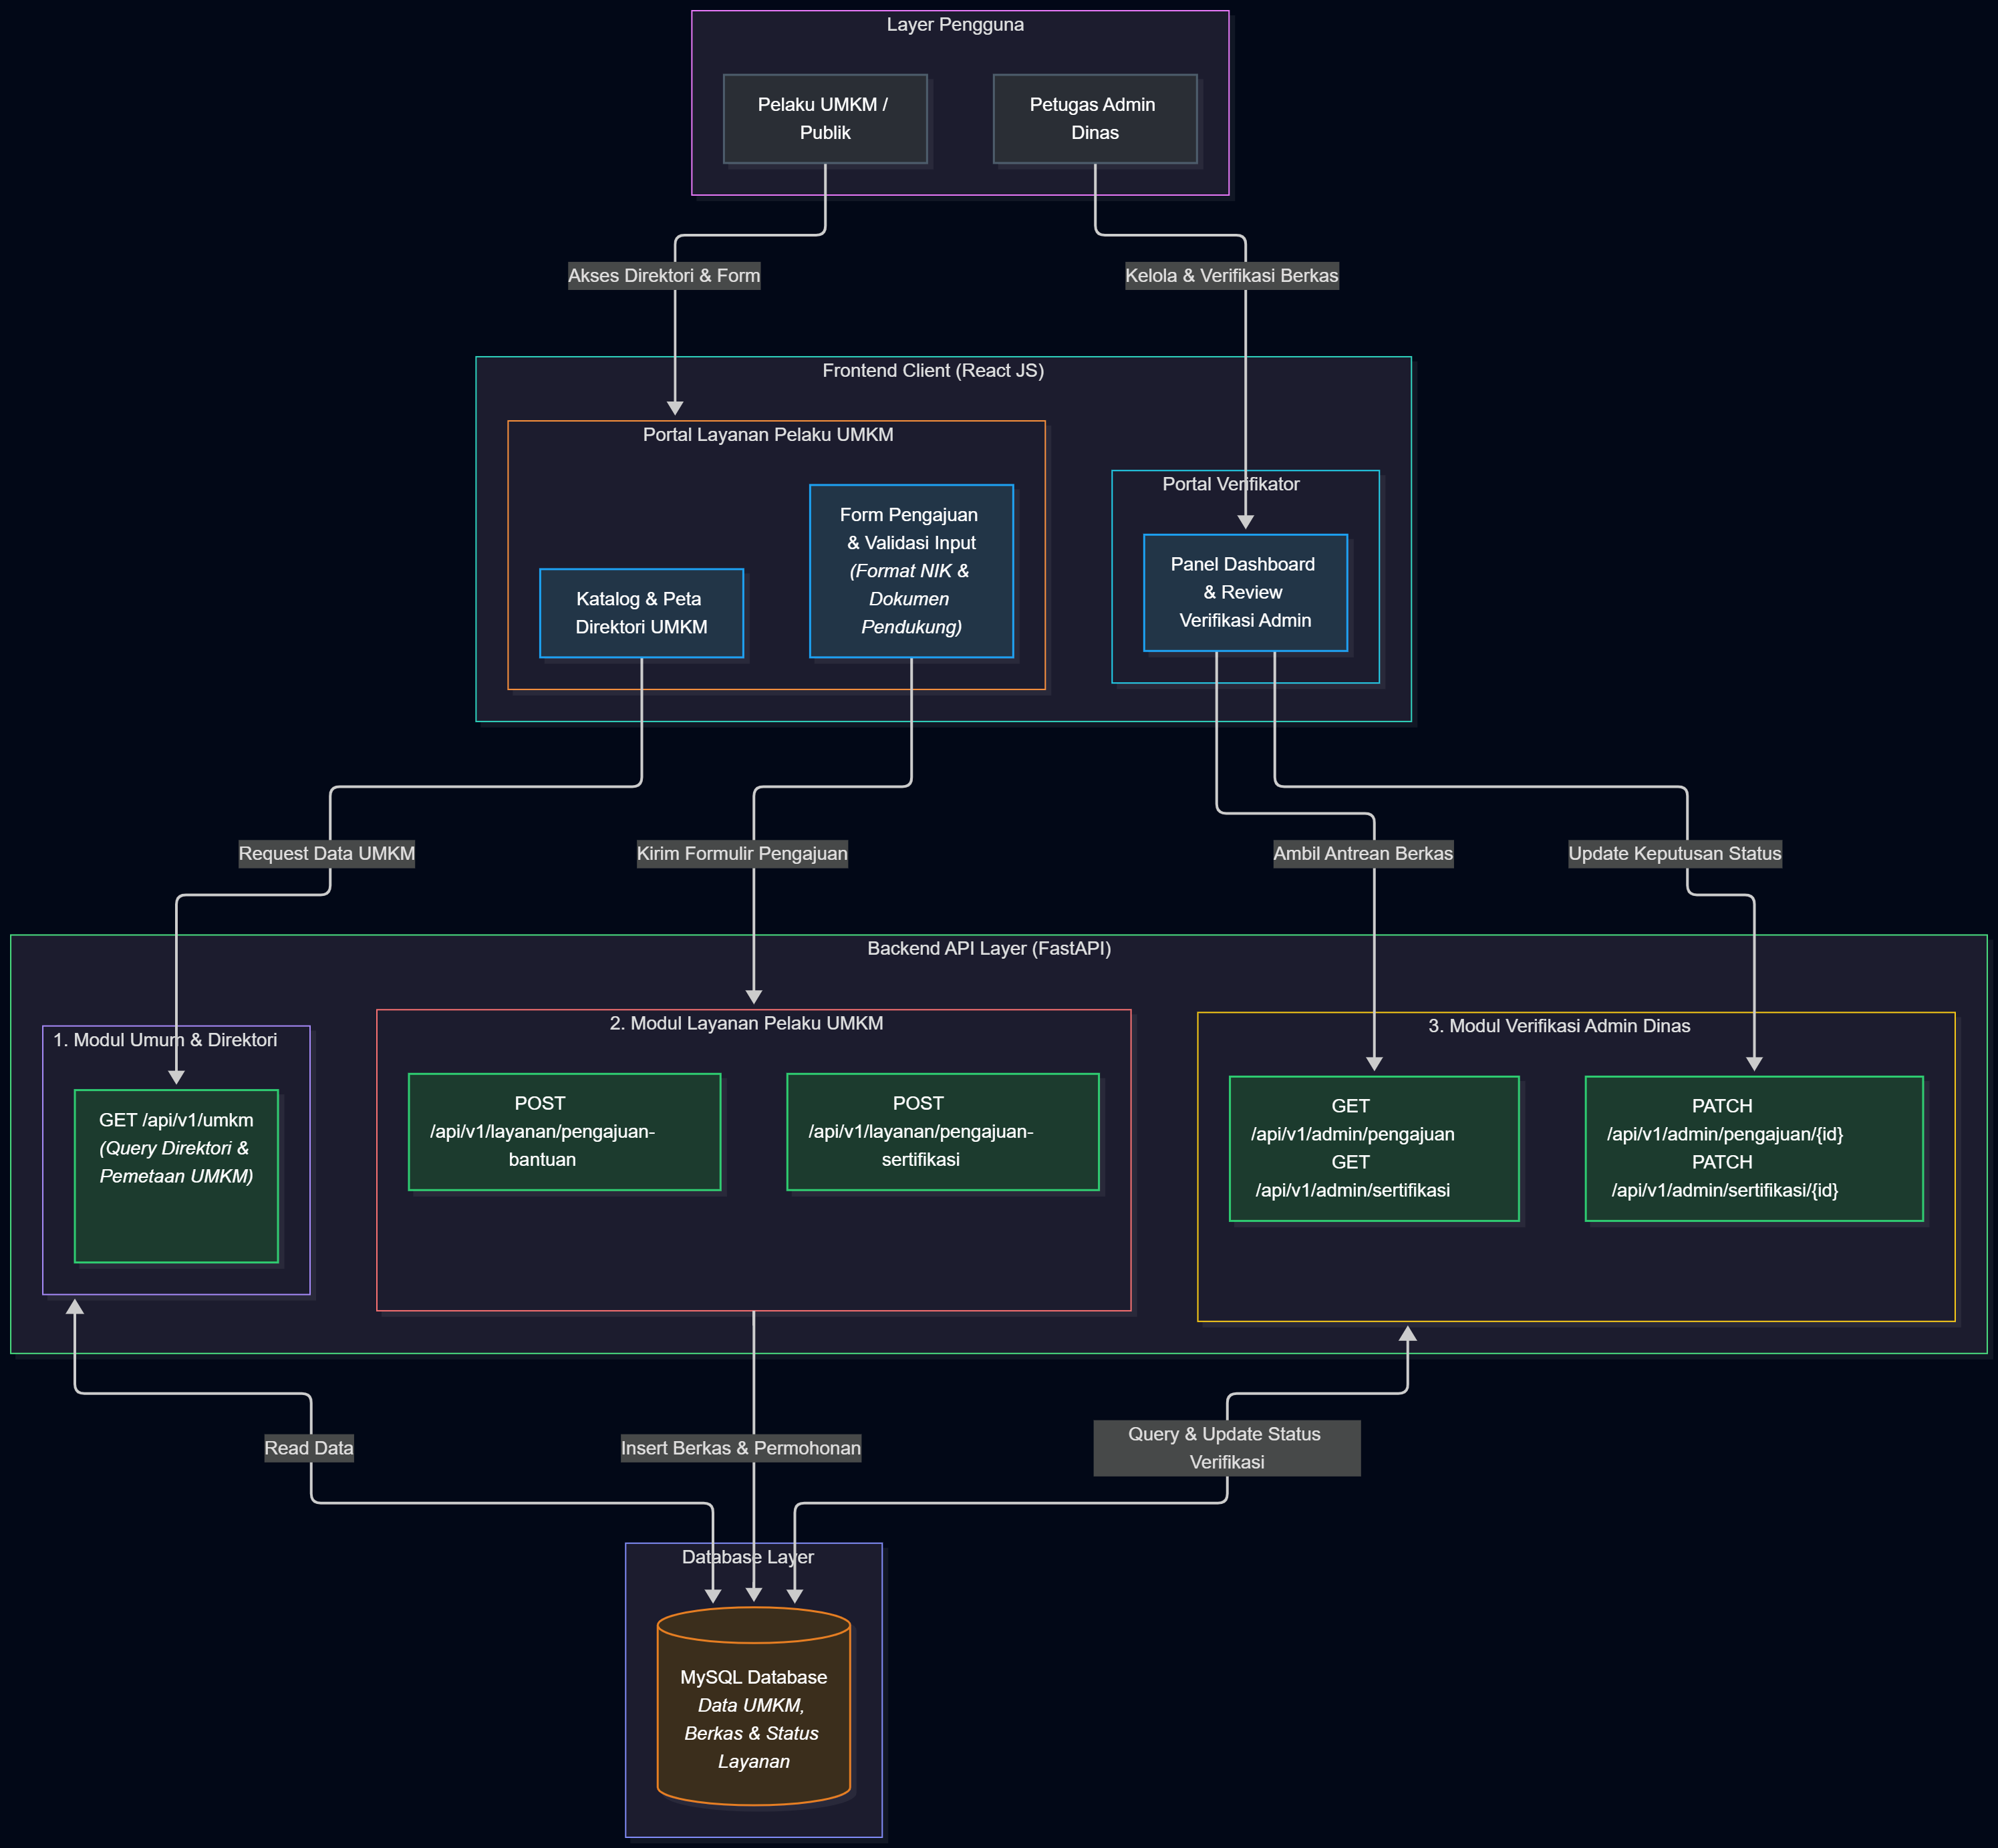
\includegraphics[width=0.88\linewidth]{gambar 2.png}
\caption{Desain Arsitektur Sistem SI-UMKM Jabar.}
\label{fig:arsitektur}
\end{figure}

\newpage

\section{Design System}
\begin{figure}[H]
\centering
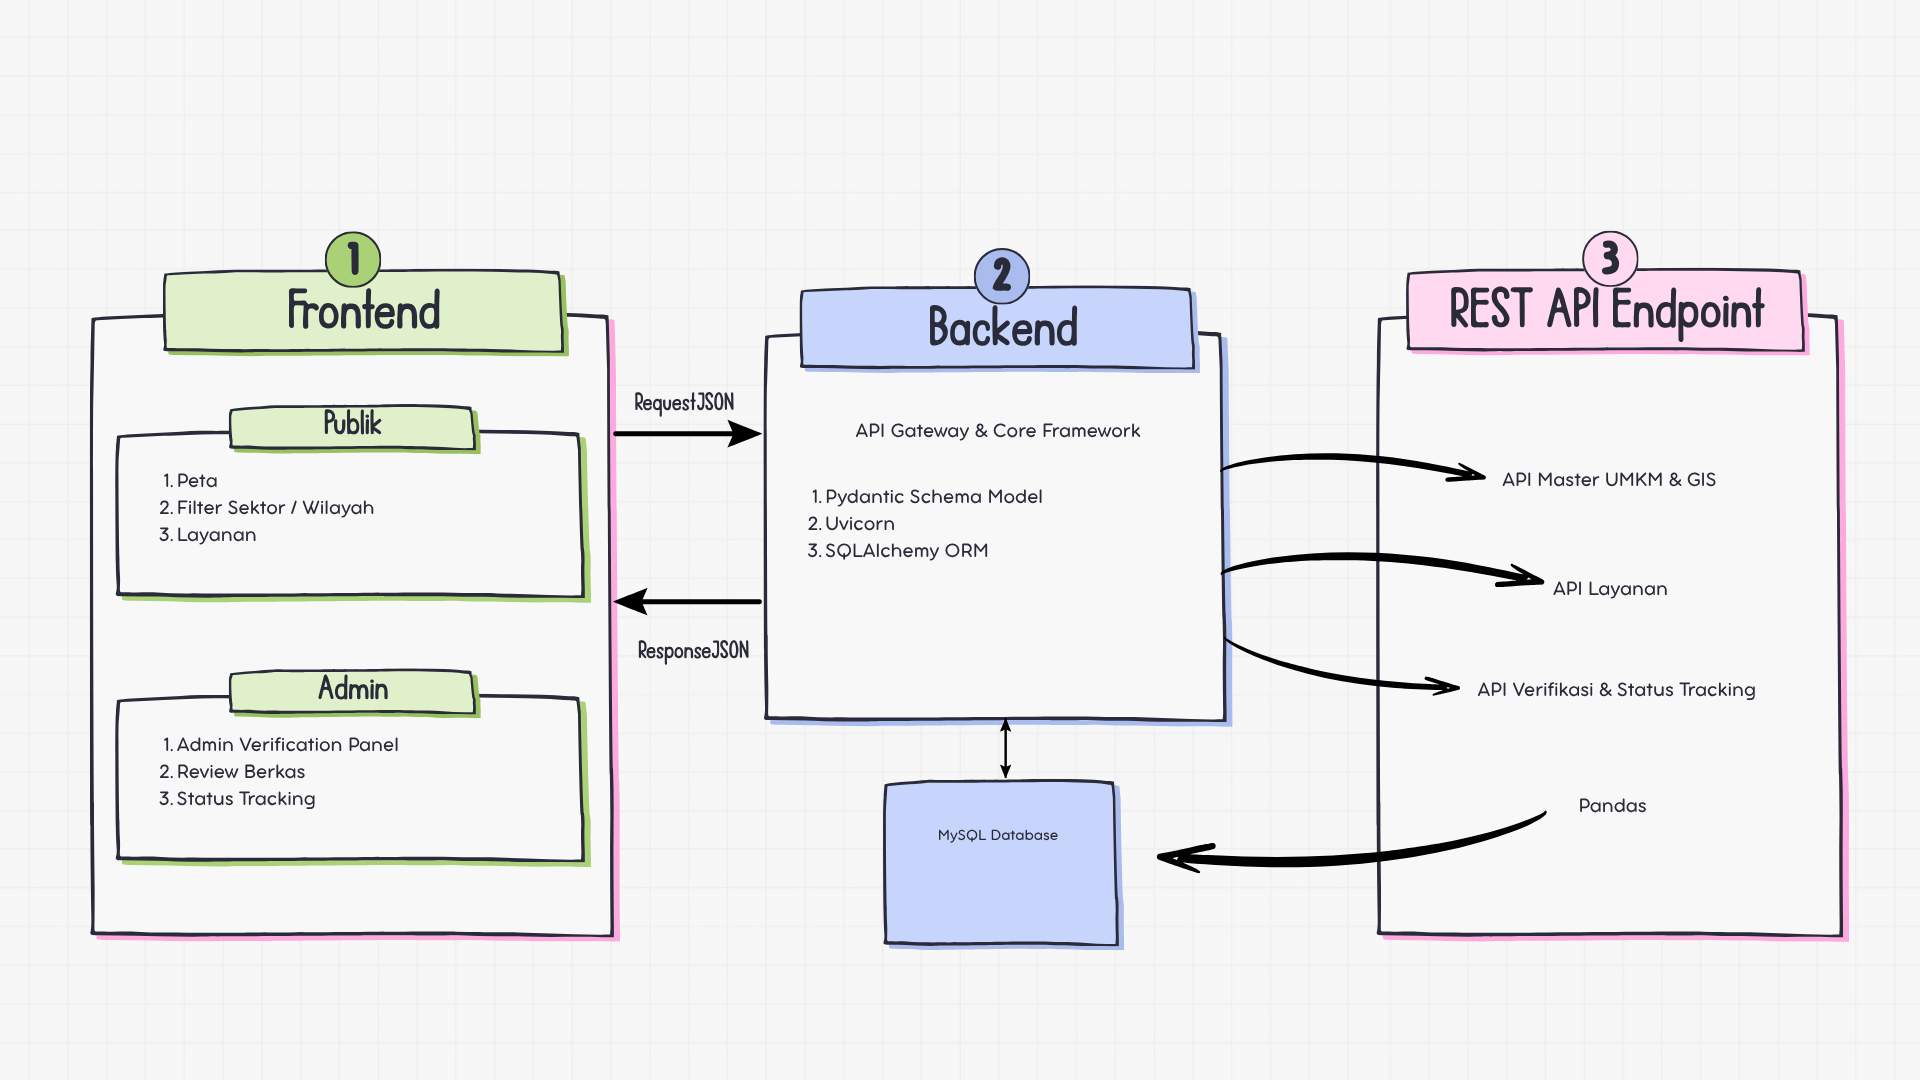
\includegraphics[width=0.88\linewidth]{gambar 3.png}
\caption{Design System Antarmuka SI-UMKM Jabar.}
\label{fig:design_system}
\end{figure}

\newpage

\section{Mockup UI - Dashboard Pengguna}
\begin{figure}[H]
\centering
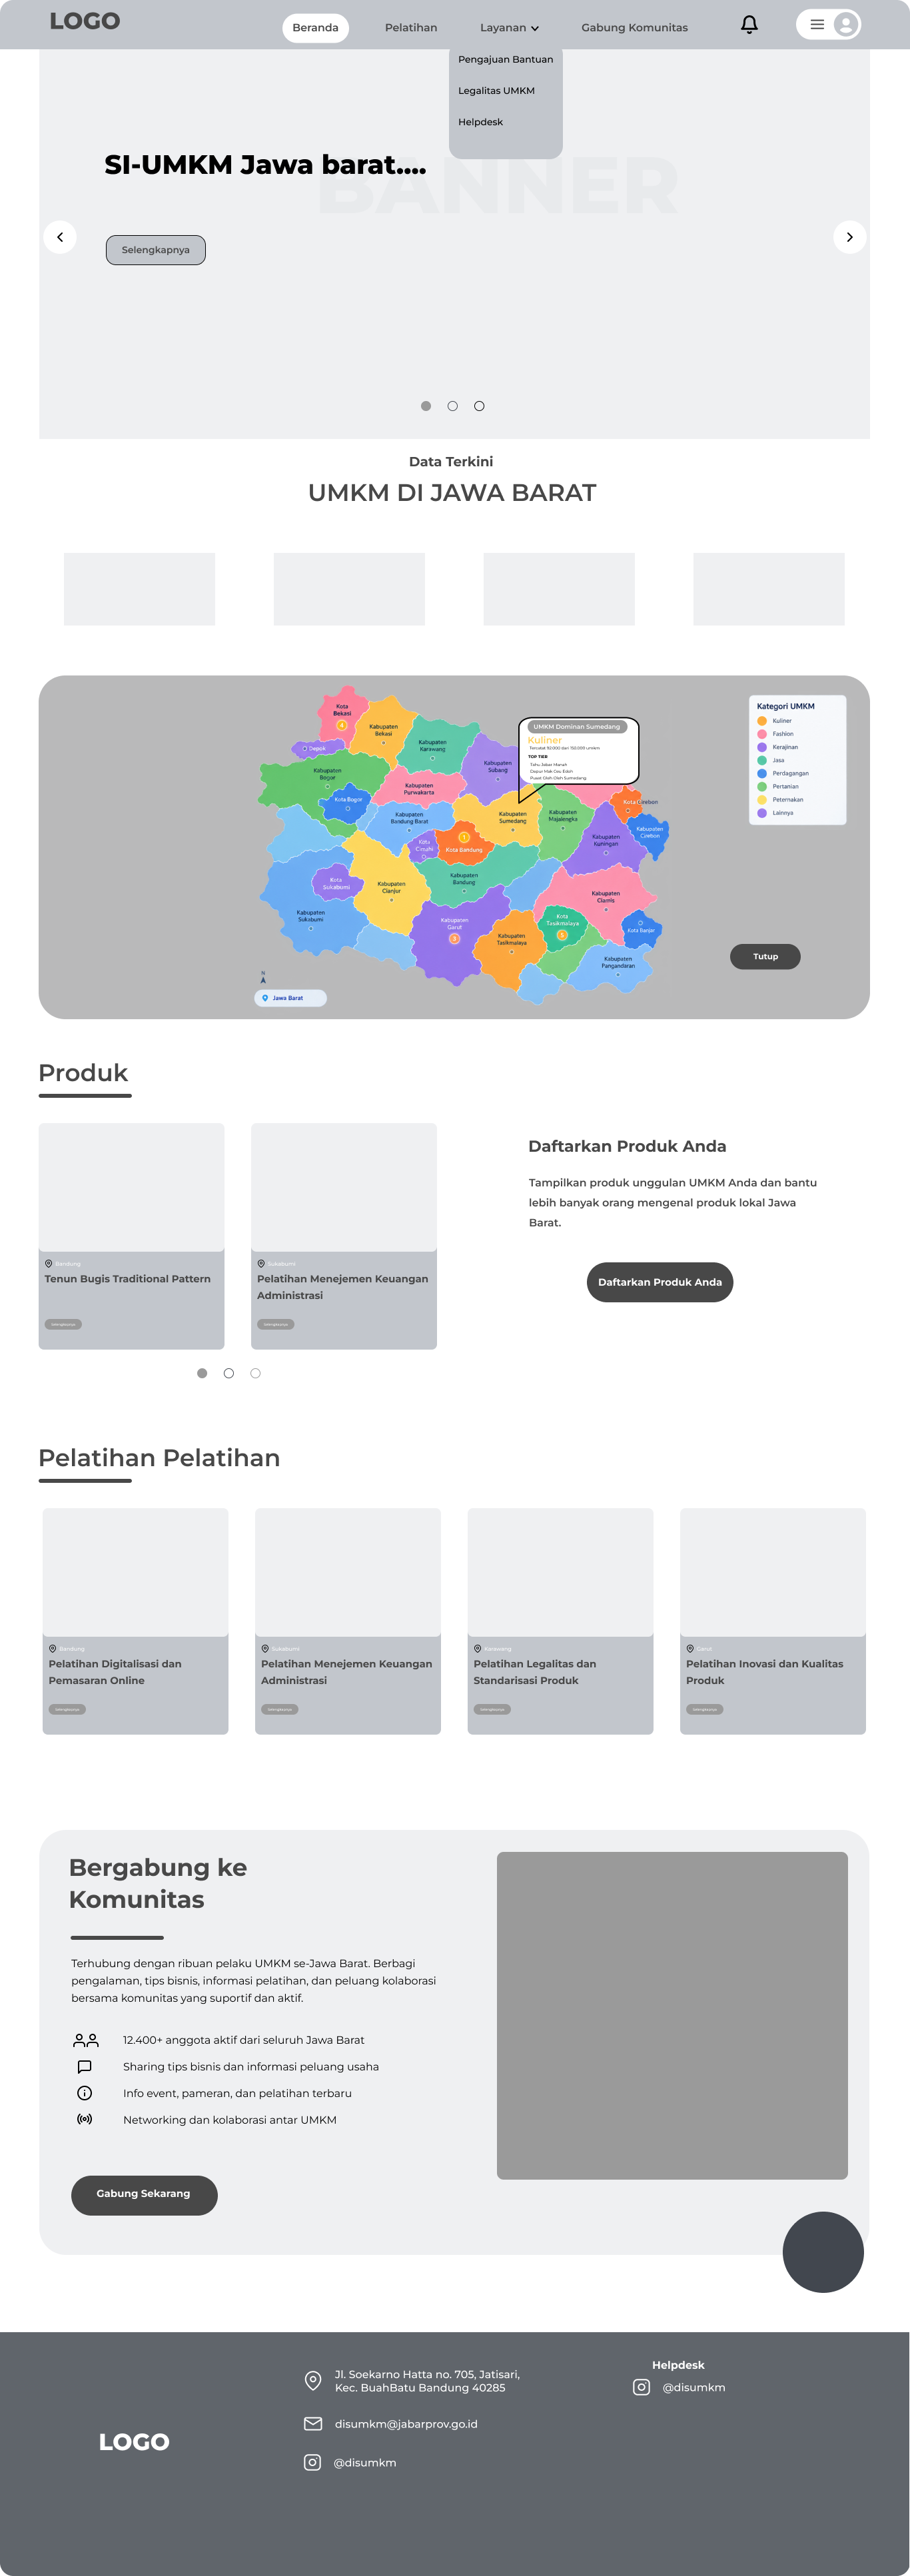
\includegraphics[width=0.85\linewidth]{gambar 4.png}
\caption{Dashboard Utama Pengguna.}
\label{fig:ui_dashboard_user}
\end{figure}

\newpage

\section{Mockup UI - Registrasi \& Login}
\begin{figure}[H]
\centering
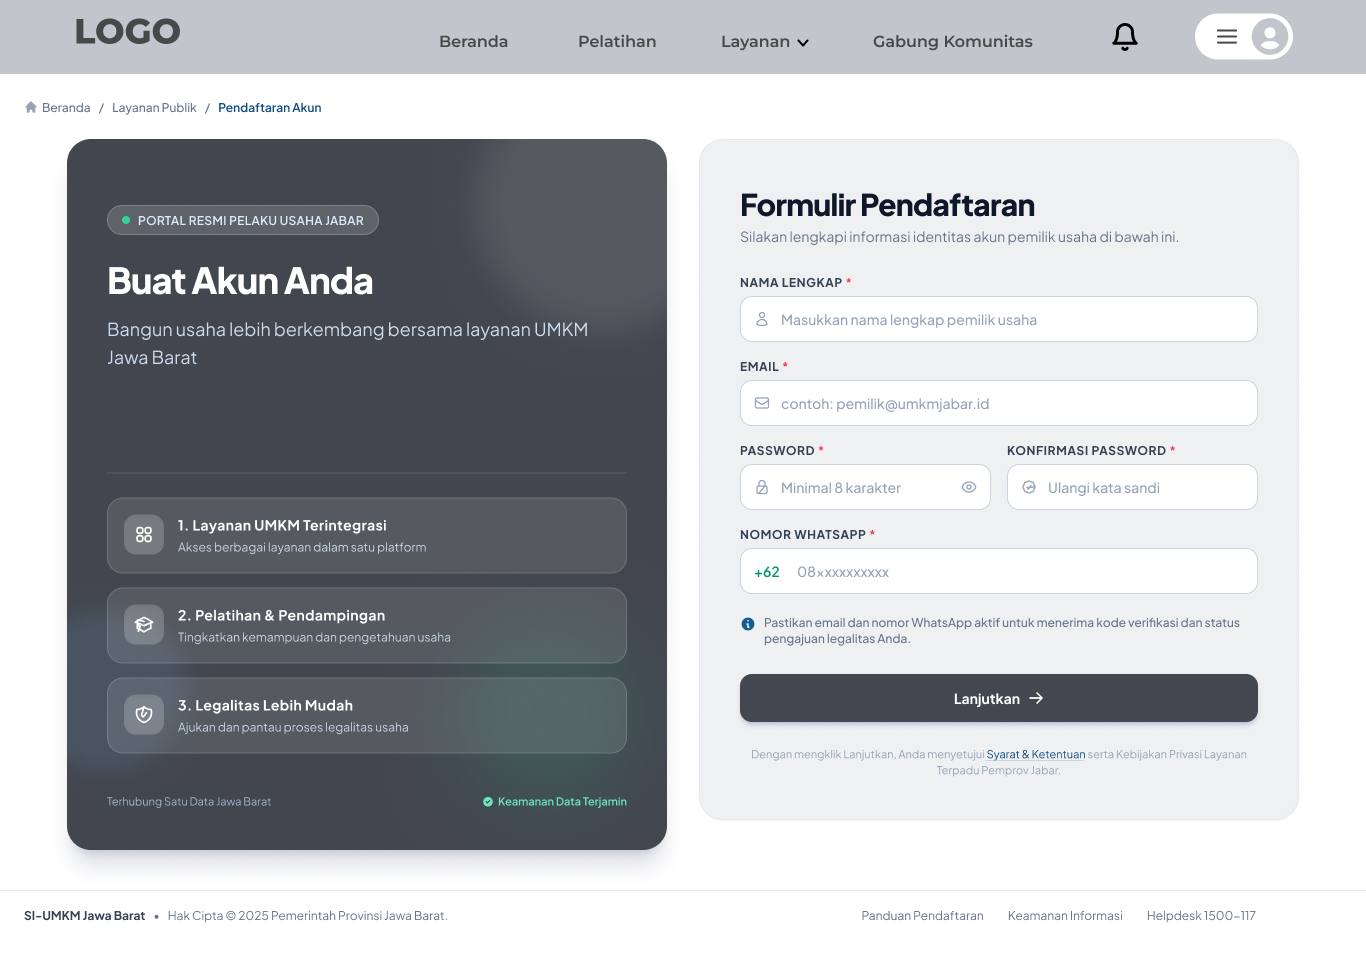
\includegraphics[width=0.85\linewidth]{gambar 5.png}
\caption{Halaman Registrasi dan Login Akun.}
\label{fig:ui_login}
\end{figure}

\newpage

\section{Mockup UI - Pengajuan Layanan Bantuan}
\begin{figure}[H]
\centering
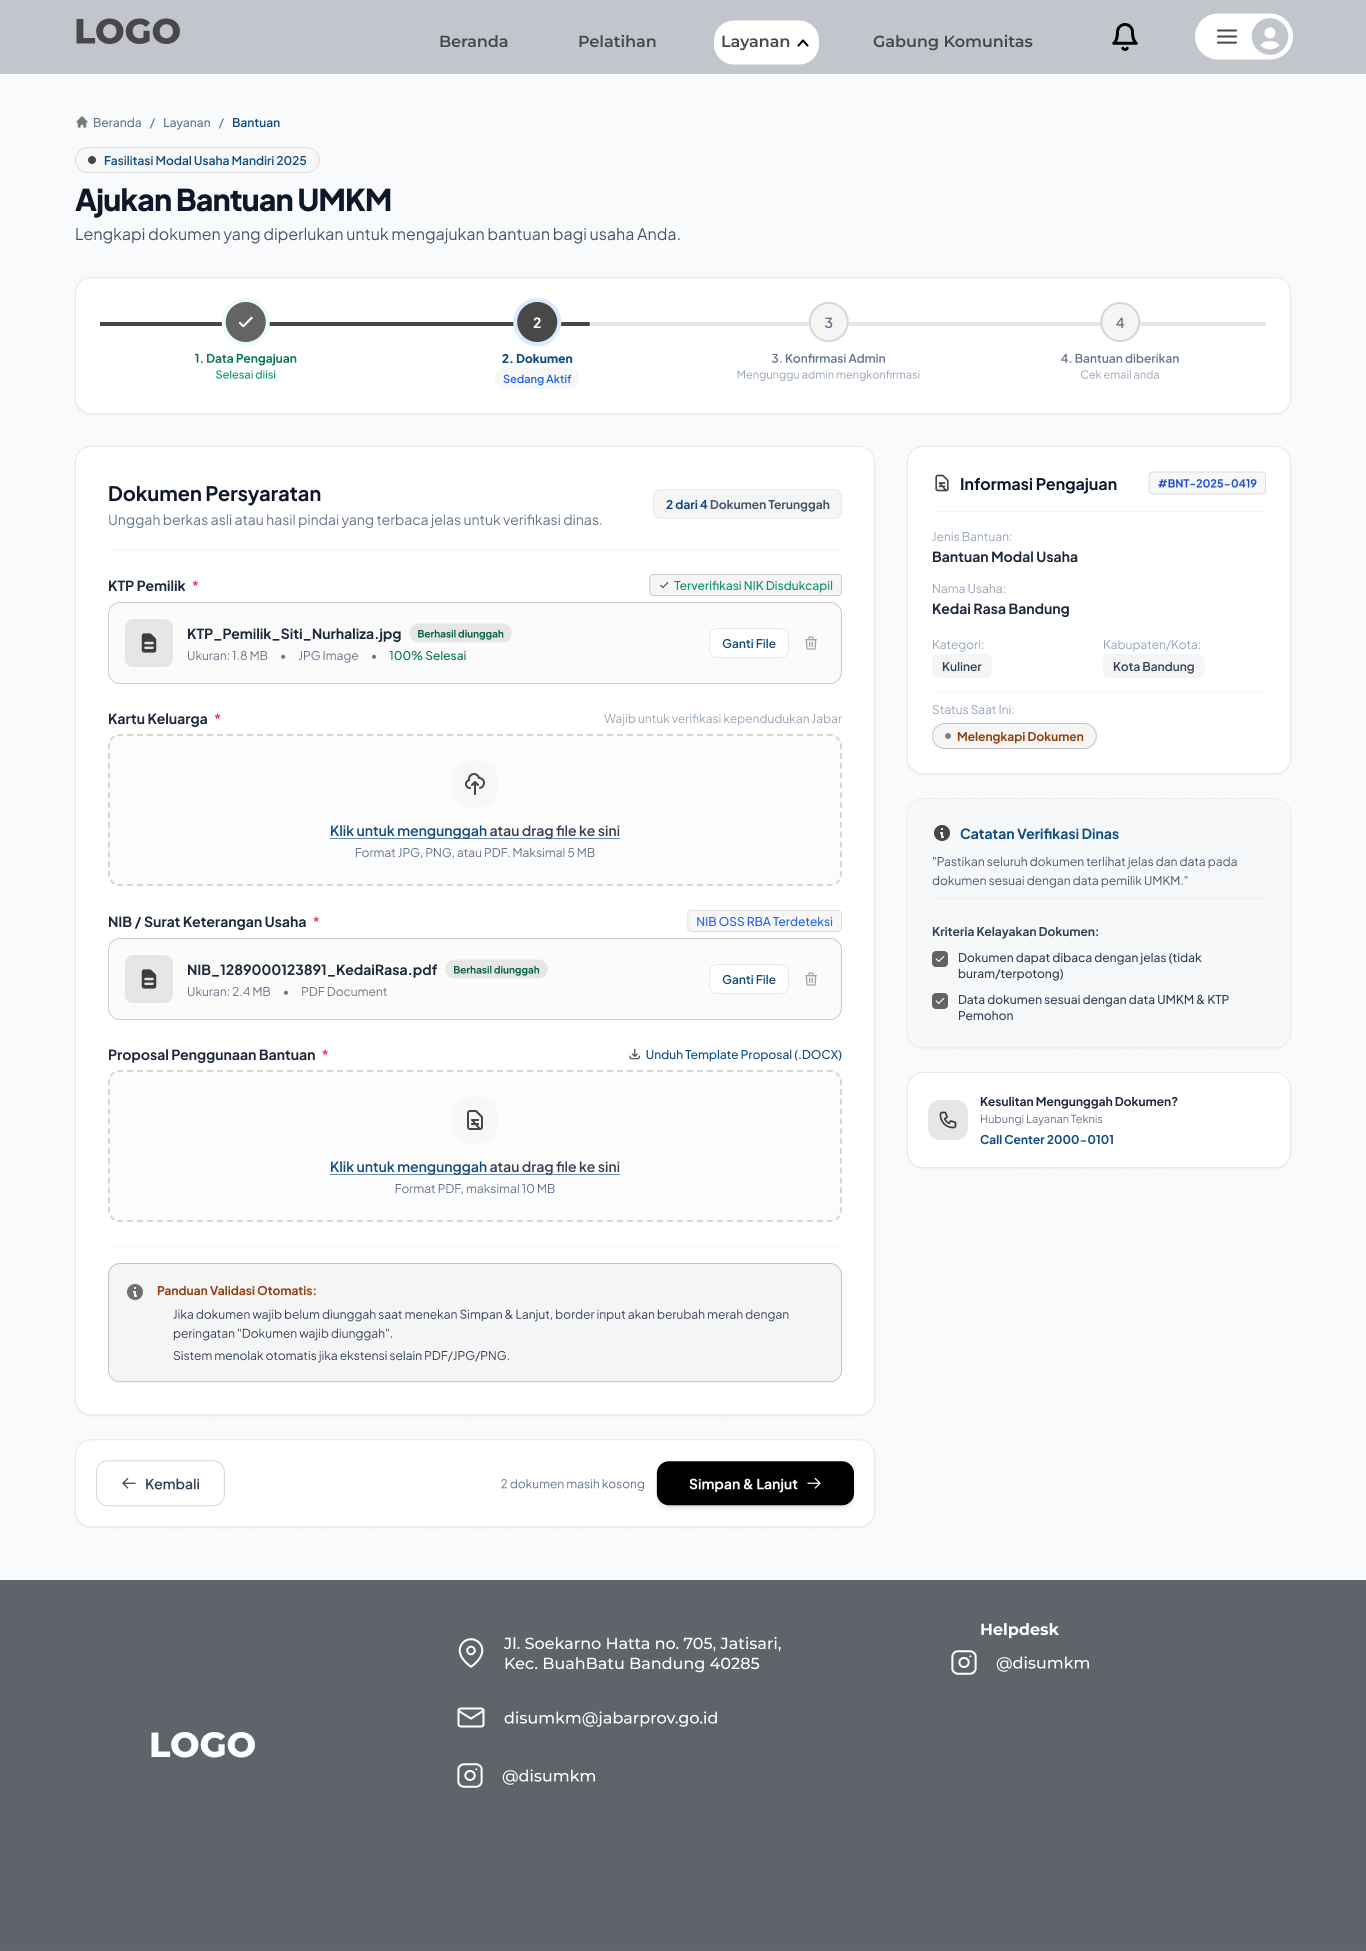
\includegraphics[width=0.85\linewidth]{gambar 6.png}
\caption{Halaman Pengajuan Layanan Bantuan UMKM.}
\label{fig:ui_bantuan}
\end{figure}

\newpage

\section{Mockup UI - Pendaftaran Pelatihan}
\begin{figure}[H]
\centering
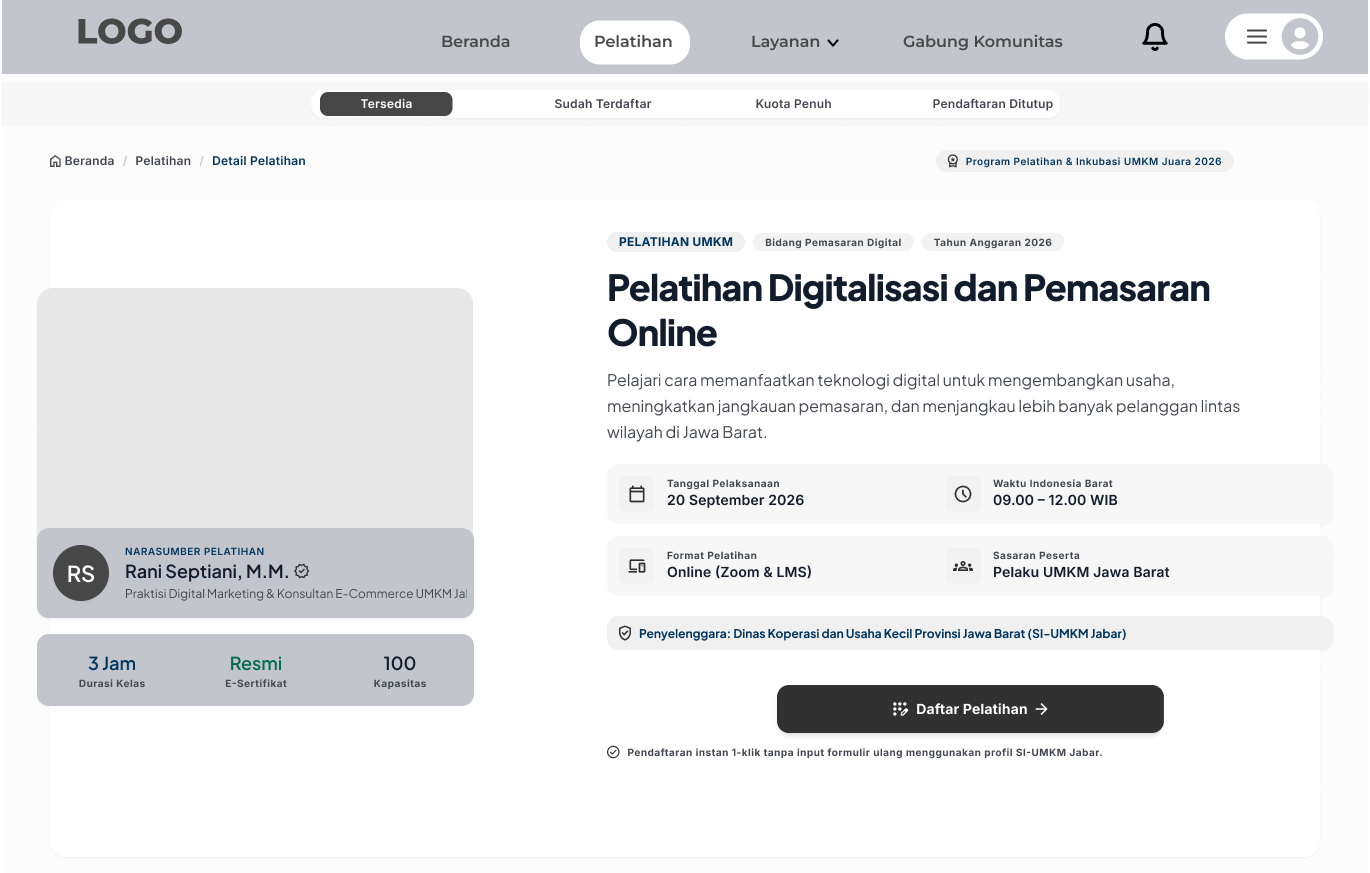
\includegraphics[width=0.85\linewidth]{gambar 7.png}
\caption{Halaman Pendaftaran Pelatihan UMKM.}
\label{fig:ui_pelatihan}
\end{figure}

\newpage

\section{Mockup UI - Dashboard Administrator}
\begin{figure}[H]
\centering
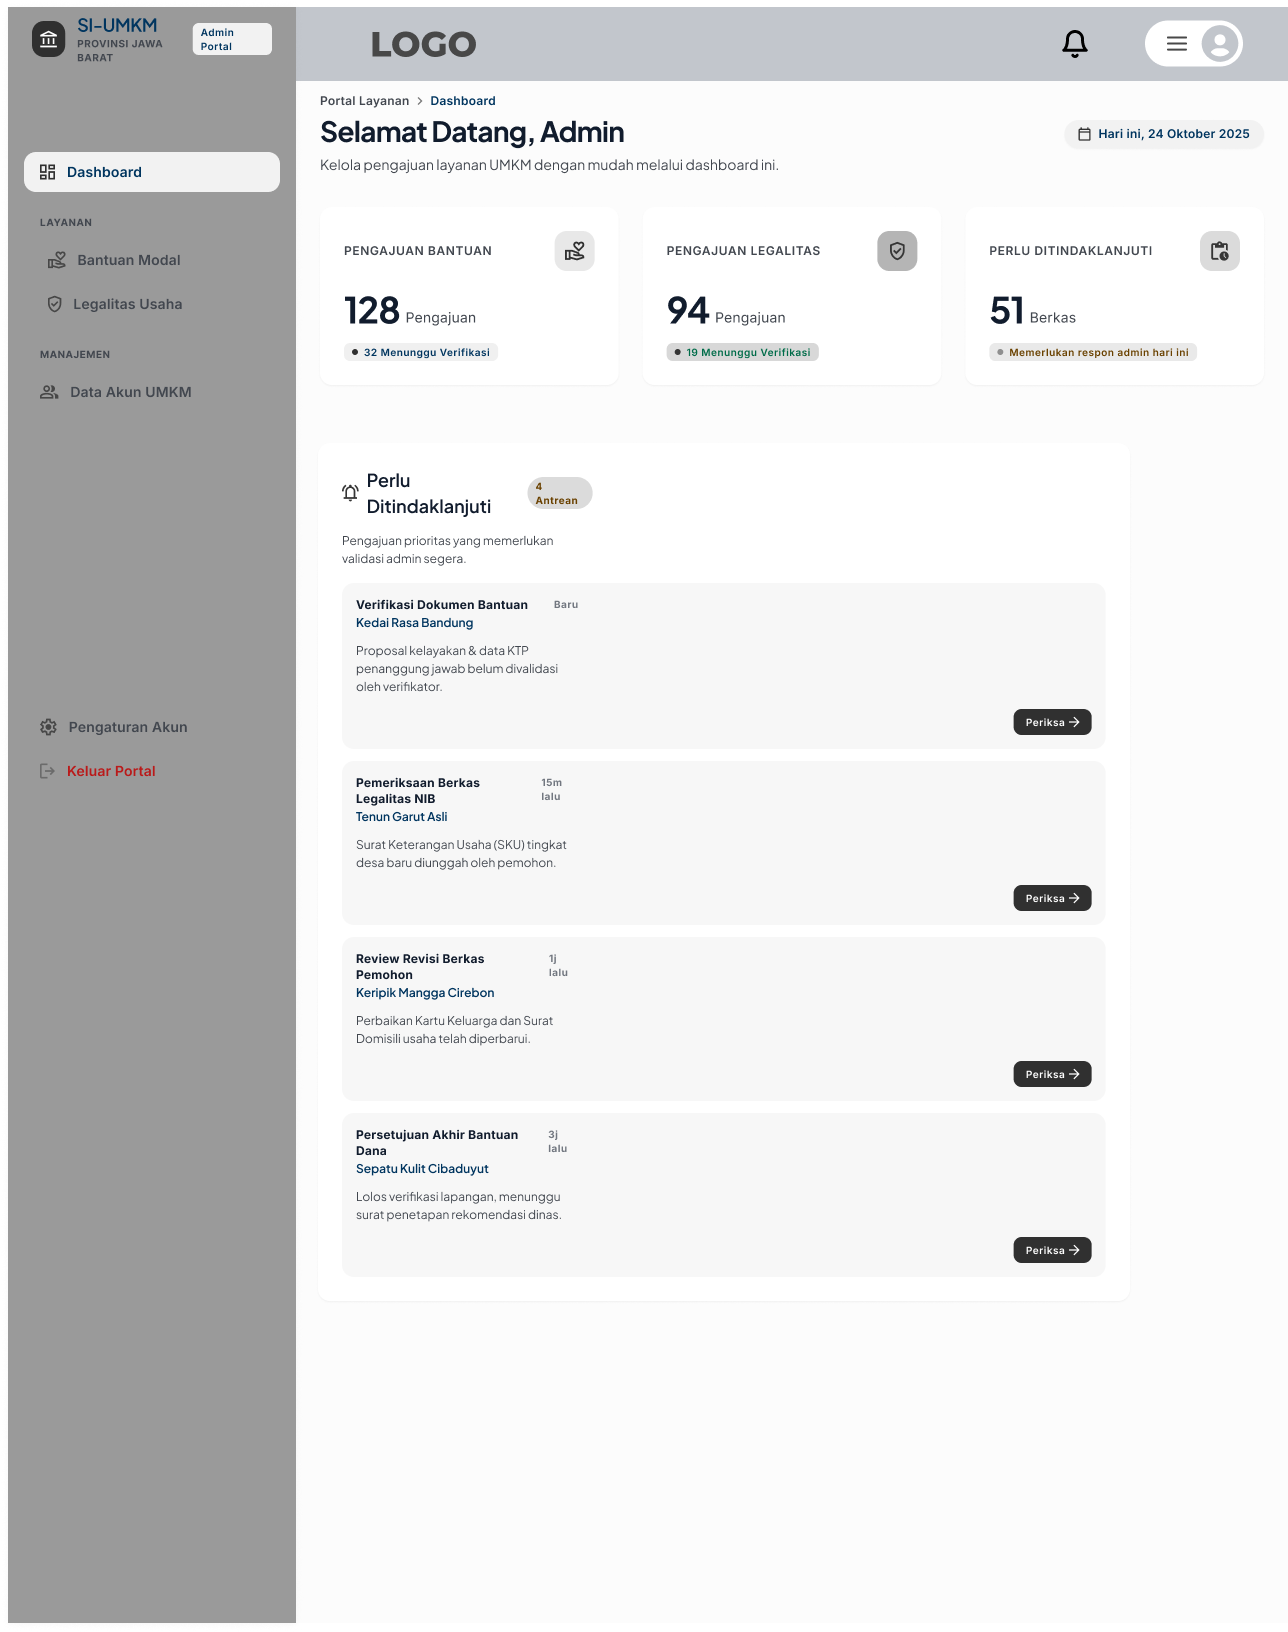
\includegraphics[width=0.85\linewidth]{gambar 8.png}
\caption{Dashboard Utama Panel Admin.}
\label{fig:ui_dashboard_admin}
\end{figure}

\newpage

\section{Mockup UI - Detail Verifikasi Berkas}
\begin{figure}[H]
\centering
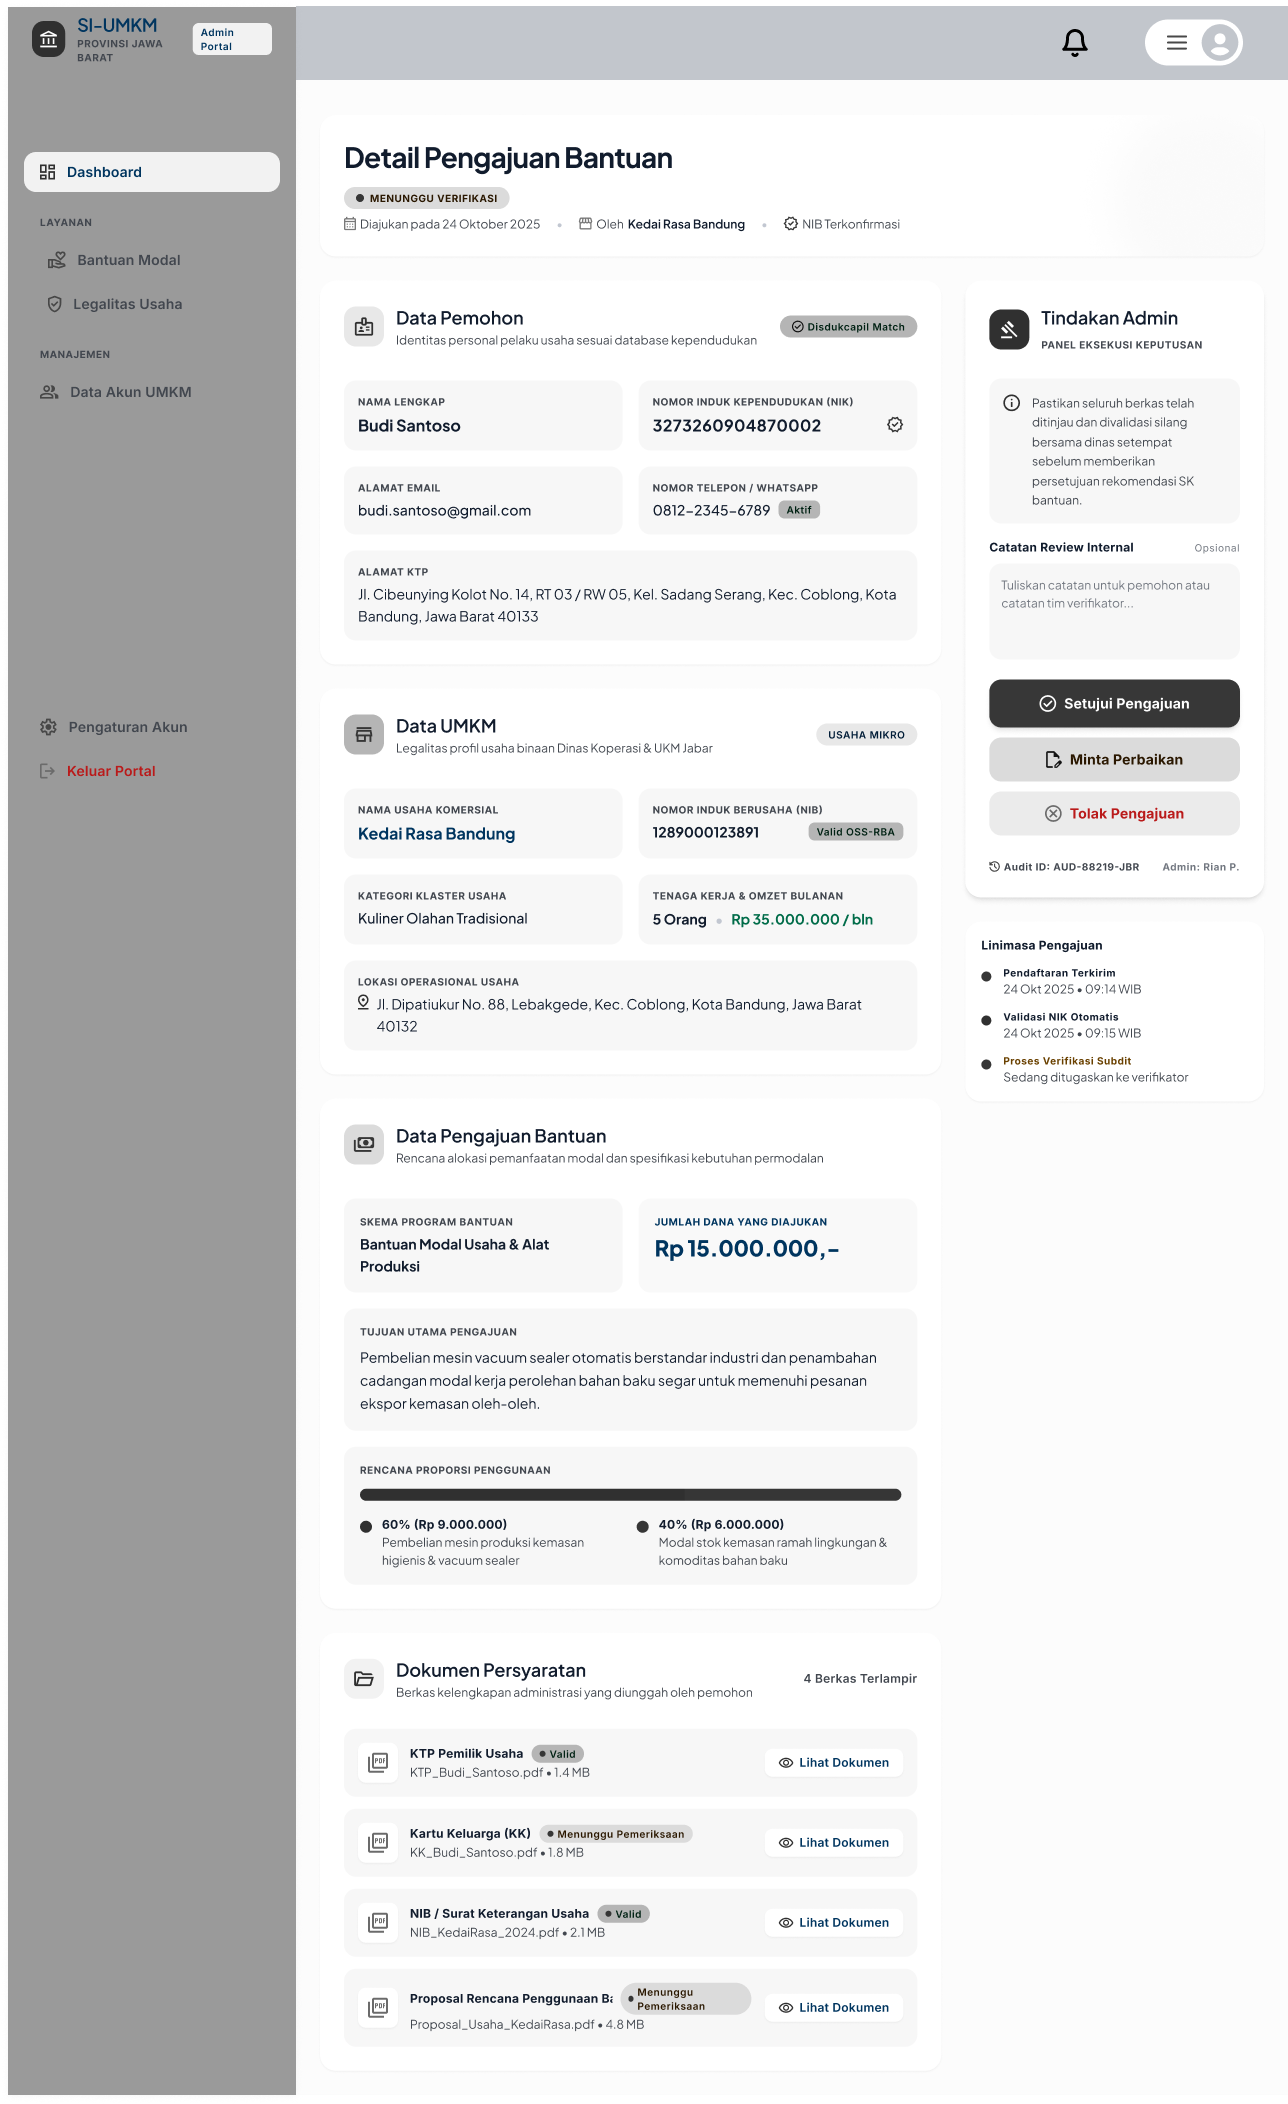
\includegraphics[width=0.85\linewidth]{gambar 9.png}
\caption{Detail Verifikasi Berkas Layanan Admin.}
\label{fig:ui_detail_admin}
\end{figure}

\newpage

\section{Alur Kerja Sistem (Flowchart)}
\begin{figure}[H]
\centering
\begin{minipage}{0.48\linewidth}
    \centering
    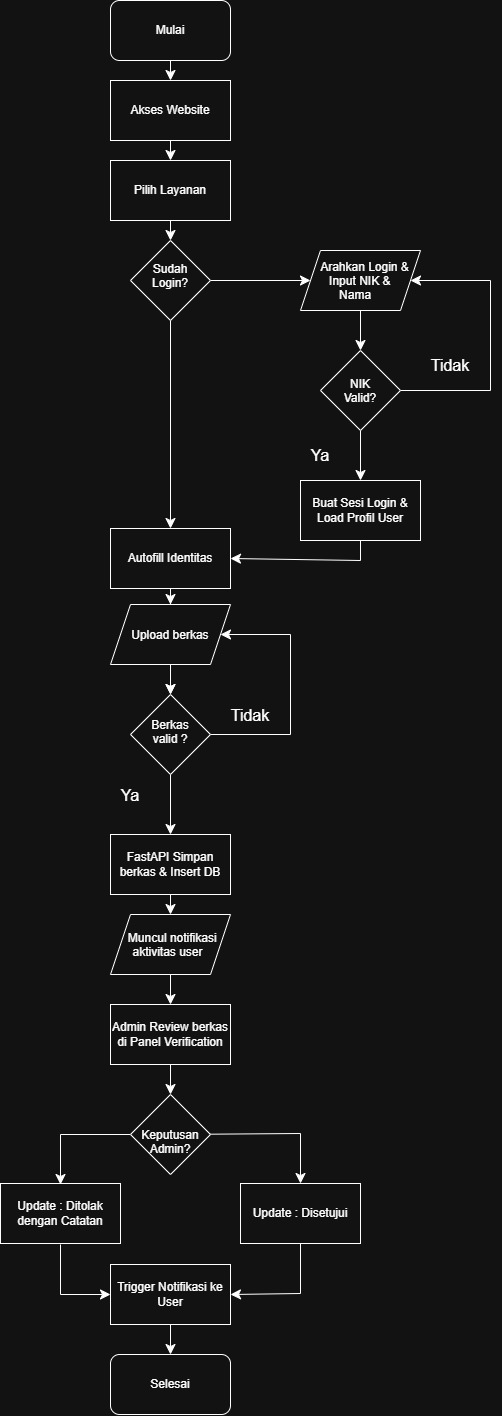
\includegraphics[height=18cm, keepaspectratio]{gambar 10.jpg}
    \caption{Flowchart Pemohon Layanan.}
    \label{fig:flowchart_user}
\end{minipage}\hfill
\begin{minipage}{0.48\linewidth}
    \centering
    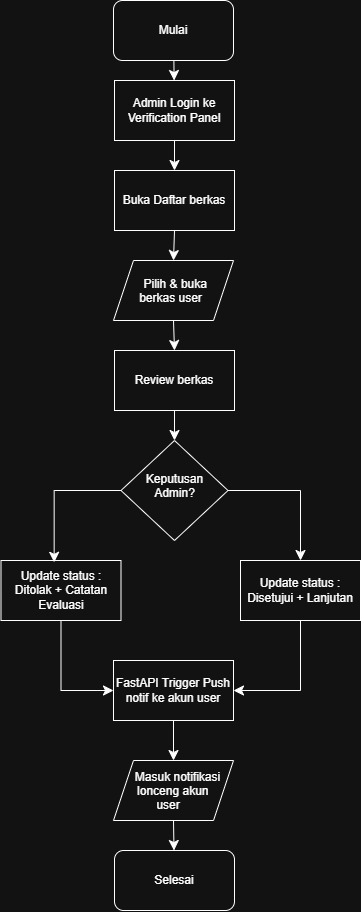
\includegraphics[height=18cm, keepaspectratio]{gambar 11.jpg}
    \caption{Flowchart Verifikator Administrator.}
    \label{fig:flowchart_admin}
\end{minipage}
\end{figure}

\newpage

\section{Pengujian Beban Server (Postman)}
\begin{figure}[H]
\centering
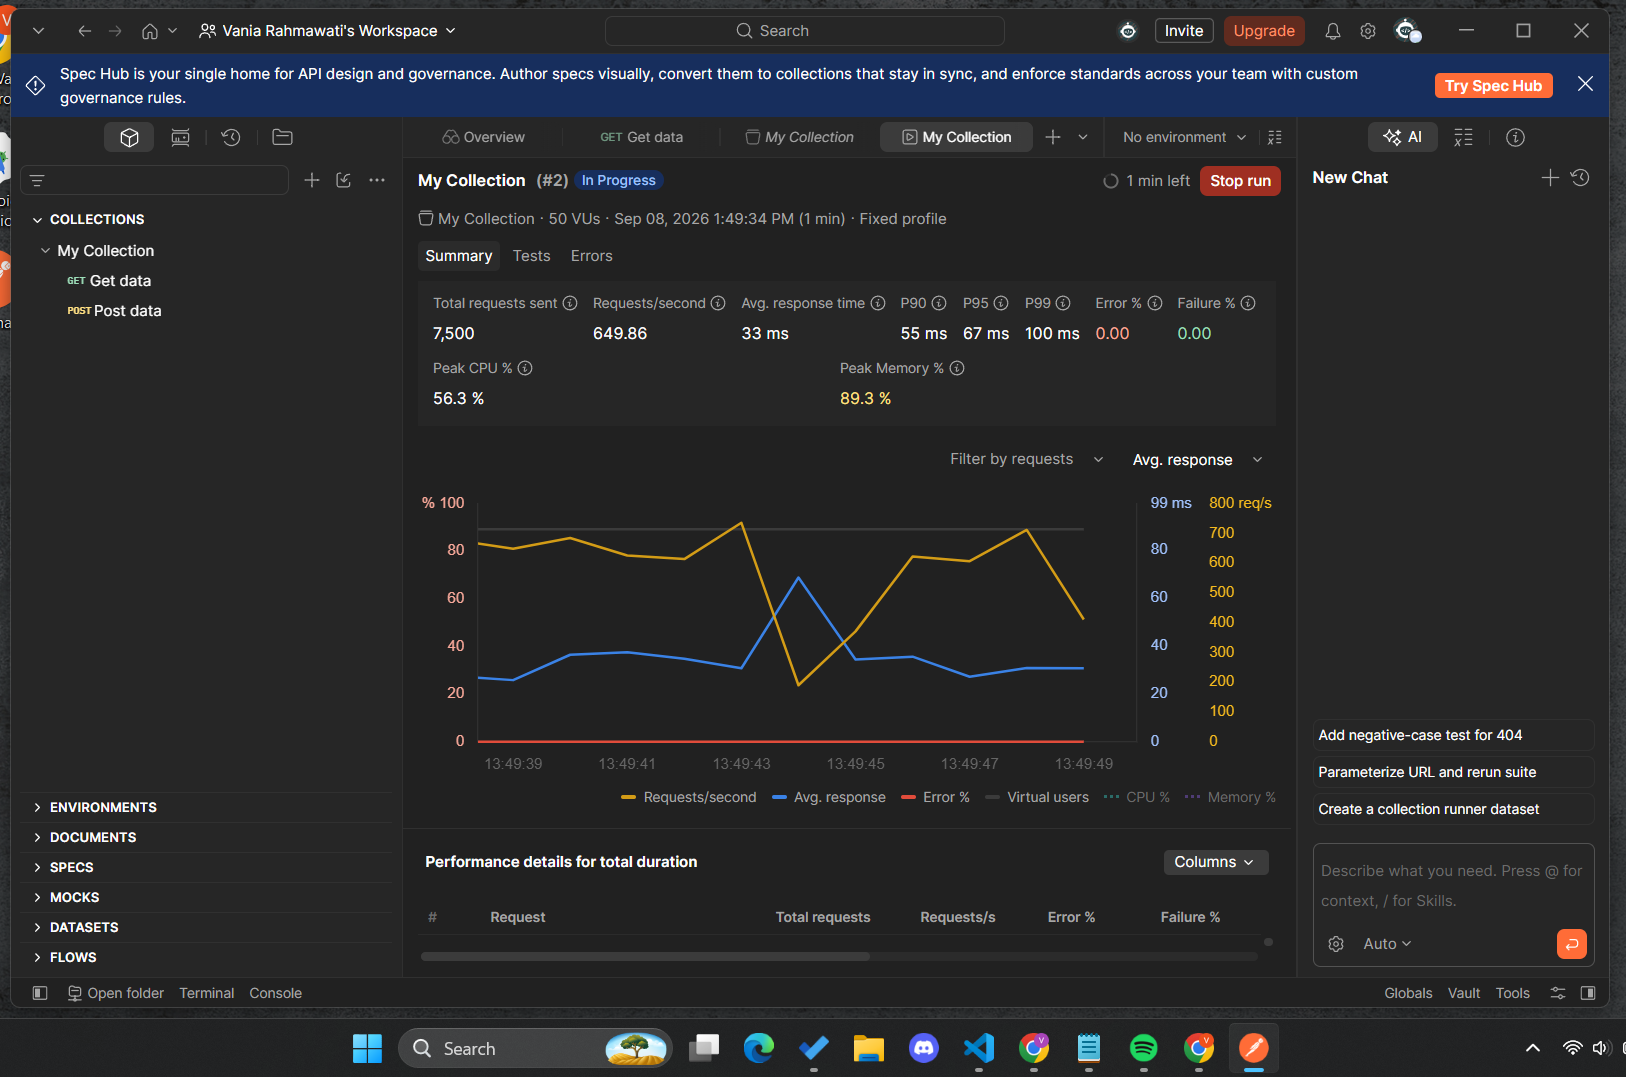
\includegraphics[width=0.88\linewidth]{gambar 12.png}
\caption{Hasil Uji Beban 50 Pengguna dalam Semenit Menggunakan Postman.}
\label{fig:postman_result}
\end{figure}

\end{document}